\chapter{Future Work}\label{ch:future_work}

This chapter presents possible improvements to the system that was not implemented by the authors of this report. This list should be of interest to other students who wish to continue work on the aSTEP multi-project and in particular the specific domain this project is concerned with.

\section{Map Matching}
In the project two different types of problems appear; one working with errors in the density estimation and one with moving people. Map matching techniques can be used to solve these problems and thereby improve the system,

\subsection{Density Estimation Error With Obstacles}
In \cref{sub:kernelDensityEstimation} we calculate the local crowd density considering points that are a maximum of the bandwidth away from the point and assume an area of a circle with a radius of the bandwidth. A problem arises with this; In \cref{fig:fenceCrowd} a crowd standing against a fence is illustrated. If a person was standing at the red point, which is the centre of the blue area illustrating the bandwidth, they would only be affected by the people south of the fence and not the absence of people north of it. If we assume a bandwidth of 5 meters, the person's perceived density would be around $1 \text{ people} / m^2$. If we calculate the density as explained in \cref{sub:kernelDensityEstimation}, with the blue area taken into consideration the density would be around $0.5 \text{ people} / m^2$.
This problem could be solved with some form of map matching that could dynamically change the area considered for each local crowd density, taking obstacles into consideration.

\begin{figure}[htbp]
\centering
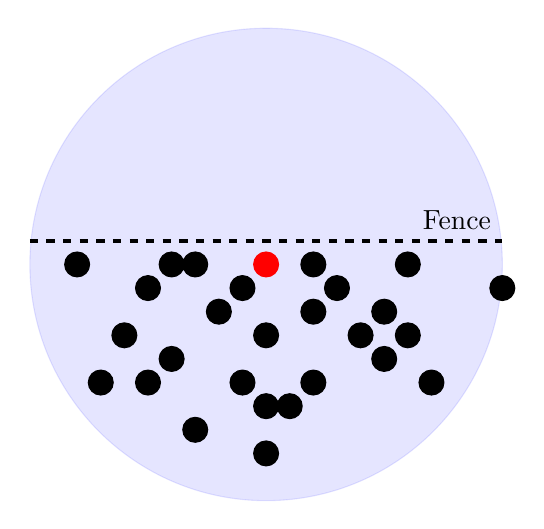
\begin{tikzpicture}[scale=3]
\coordinate (A) at (0,-0.1);
\coordinate (B) at (0.2,-0.1);
\coordinate (C) at (0.4,-0.4);
\coordinate (D) at (-0.1,-0.3);
\coordinate (E) at (-0.5,-0.6);
\coordinate (F) at (1,-0.2);
\coordinate (G) at (-0.4,-0.5);
\coordinate (H) at (0.7,-0.6);
\coordinate (I) at (0.2,-0.3);
\coordinate (J) at (0.6,-0.4);
\coordinate (K) at (-0.7,-0.6);
\coordinate (L) at (-0.3,-0.1);
\coordinate (M) at (-0.6,-0.4);
\coordinate (N) at (-0.8,-0.1);
\coordinate (O) at (-0.4,-0.1);
\coordinate (P) at (-0.5,-0.2);
\coordinate (Q) at (-0.2,-0.3);
\coordinate (R) at (-0.1,-0.6);
\coordinate (S) at (-0.1,-0.2);
\coordinate (T) at (-0,-0.7);
\coordinate (U) at (-0,-0.4);
\coordinate (V) at (0.2,-0.6);
\coordinate (W) at (0.1,-0.7);
\coordinate (X) at (-0.3,-0.8);
\coordinate (Y) at (0.5,-0.5);
\coordinate (Z) at (-0,-0.9);
\coordinate (AA) at (0.3,-0.2);
\coordinate (AB) at (0.5,-0.3);
\coordinate (AC) at (0.6,-0.1);

\filldraw[color = blue, opacity=0.1]
(A) circle (1);

\filldraw
(B) circle (1.5pt)
(C) circle (1.5pt)
(E) circle (1.5pt)
(F) circle (1.5pt)
(G) circle (1.5pt)
(H) circle (1.5pt)
(I) circle (1.5pt)
(J) circle (1.5pt)
(K) circle (1.5pt)
(L) circle (1.5pt)
(M) circle (1.5pt)
(N) circle (1.5pt)
(O) circle (1.5pt)
(P) circle (1.5pt)
(Q) circle (1.5pt)
(R) circle (1.5pt)
(S) circle (1.5pt)
(T) circle (1.5pt)
(U) circle (1.5pt)
(V) circle (1.5pt)
(W) circle (1.5pt)
(X) circle (1.5pt)
(Y) circle (1.5pt)
(Z) circle (1.5pt)
(AA) circle (1.5pt)
(AB) circle (1.5pt)
(AC) circle (1.5pt);

\filldraw[color = red]
(A) circle (1.5pt);

\draw[ultra thick, dashed] (-1,0) -- (1,0) node[above left] {Fence};
\end{tikzpicture}
\caption{Crowd standing against a fence.}
\label{fig:fenceCrowd}
\end{figure}

\subsection{Moving people}
Due to the imprecision of real world data a person can jump back and forth between two points on a map that are separated by an obstacle when they in reality are just standing on one side of the obstacle. 

Some of these issues could be eliminates using map matching techniques. If people moving towards an obstacle reach the obstacle and stop or move along it, any observation received from the opposite side of the obstacle could be projected to the correct side. This behaviour should be defined in terms of some form of distance where this projection should not happen in case of errors in the map data.

\section{Warning System}
As Leif Bjørn proposed in \cref{sub:telia_parken_meeting}, a warning system would be desirable. With such an addition in place, the system is able to determine that a crowd situation can  evolve to be of a particular dangerous form, To perform such an analysis, prior incidents could be considered as a form of training data. This could also be implemented as another overlay highlighting areas when specific threshold values are satisfied. It would be useful to base these values on the levels of hazard defined in \cref{subsec:levelsOfHazard}.

\section{Statistics}
Being able to monitor different statistics such as a person count, would help the user determine how much they can rely on the system at the moment. A person count in this context refers to the amount of people that the system is able to locate at the moment. If the system is only keeping track of 5000 people at a festival, but the total number of visitors is 50000, the system is only able to provide estimates on crowd condtitions based on 10\% of the visitors. It could also be interesting to be able to see historical statistics on for example the person count to be able to analyse the cause of specific incidents.

\section{Navigation}
The requirements of the second sprint, presented in \cref{sec:s2_reqs}, describes the feature of user navigation. The feature was priorities as \enquote{could have} at the time, as it did not fit the direction of the project.

The feature is similar to existing navigation systems for cars. These systems take traffic into consideration when guiding the user to their destination using the optimal route. In the context of events, the traffic is often large groups of people blocking pathways. The system should be able to guide users through event areas using the fastest route. This can be critical for navigating medical personnel to injured people as fast and accurate as possible.

\section{Prediction of Crowd Conditions}
The system can currently only estimate crowd conditions going back in time. It would be useful for crowd safety/management personnel to be able to also see what the crowd conditions will be like in the near future. This could be used to significantly mitigate the risk of crowd disasters by allowing crowd safety personnel to actively take preventive action.

This feature can be implemented by analysing the current crowd condition trend, and possibly also teach the system which factors caused prior incidents to happen.

\section{User Placeable Markers}
The idea is for guards to be able to place markers on the map using their smartphones. A marker could have a note saying \enquote{Fight here}. The operators of the system would then be able to see this marker and its location, and take appropriate action.

\section{Switch From Mapbox.js to Leaflet}
Although Mapbox.js is an open-source library, it needs an access token issued from Mapbox in order to function. There is no particular reason that Leaflet can not be used directly, instead of Mapbox.js, other than Mapbox.js having more features. This would make the mapping functionality independent on the commercial company Mapbox.

\section{Better Selection of Points to Analyse}
As described in \cref{s3:select_points} the analyser divides the area to analyse into a grid of hexagons. This means that the number of points increases quadratically in the area to analyse.  This approach does obviously not scale well as the area to analyse increases. By naively selecting all points in a grid to analyse, many wasteful computations are made, since most of the time there are no people in the area of the hexagons.

This problem can be solved by only selecting points to analyse that have people within the bandwidth.